%%%%%%%%%%

In the standard KID readout scheme, each pixel is excited using a fixed tone at its resonant frequency. The signal transmitted past the detector is compared to a reference copy of the excitation signal to get its in-phase ($I$) and quadrature ($Q$) components. From these it is then necessary to estimate the corresponding shift in resonance frequency $f_0$ of the detector, because this is the physical property directly related to the incoming optical power: $\delta f_0 \propto \delta P_{opt} $ for low values of $\delta P_{opt} $ (\cite{Swenson2010}).
Finding a reliable way to evaluate $f_0(t)$ starting from $I(t)$ and $Q(t)$ represents a challenge, and this is especially true in the case of ground-based experiments, as these have to cope with the effects induced by the variations in atmospheric opacity. To improve the photometric reproducibility, we have developed a measurement process which is described in the next subsection.

\subsection{Modulated Readout}\label{REU}
\label{sec:rfdidq}

For the \NIKA\ detectors an innovative readout technique has been developed, which has been succesfully tested during the 2011 run and adopted for all the following campaigns. The details of this technique are described in \cite{Calvo2013}. Briefly, the underlying idea is to replace the standard excitation of the detectors, which uses a fixed tone, with a new excitation based on two different frequencies. We achieve this by modulating the local oscillator signal between two values, separated by $\delta f_{LO}$, in order to generate two tones, one just above ($f_+ = f_0 + \delta f_{LO}/2$) and one just below ($f_- = f_0 - \delta f{LO}/2$) the detector resonant frequency. The modulation is carried out at about $1~kHz$, synchronously to the FPGA sampling of the signal. Thus, each raw data point, which is sent to the acquisition software at a rate of 23.842~Hz, is composed of the values $(I(t), Q(t))$ of each pixel, as well as the corresponding differential values
\begin{equation}
\left(\frac{dI}{df}(t), \frac{dQ}{df}(t)\right) = \left(\frac{I(f_+)-I(f_-)}{\delta f_{LO}}, \frac{Q(f_+)-Q(f_-)}{\delta f_{LO}}\right).
\label{eq:dIdQ}
\end{equation}
If a variation $(\Delta I(t), \Delta Q(t))$ is observed between successive points, it is possible to estimate the corresponding shift in the resonant frequency, $\Delta f_0(t)$, by projecting $(\Delta I(t), \Delta Q(t))$ along the gradient found using equation \ref{eq:dIdQ}:
\begin{equation}
\Delta \hat{f_{0}}(t) = \frac{\left(\Delta I(t), \Delta Q(t)\right)\cdot\left(dI/df(t), dQ/df(t)\right)}{\left(dI/df(t), dQ/df(t)\right)^2}\cdot\delta f_{LO}.
\label{eq:RFdIdQ}
\end{equation}
We use the name \emph{RFdIdQ} to refer to this estimate of $\Delta f_0$.


\begin{figure}[t!]
\begin{center}
\includegraphics[bb = 132 256 450 568,width=7cm, clip]{figures/fig_resoCircle.eps}
\end{center}
  \caption{Representation in the I-Q plane of a sweep around a resonance. The measure of the angles $\varphi$ and $\vartheta$ can be carried out for each acquired point thanks to the modulated readout technique. On resonance, one gets $\vartheta = 0$}
\label{fig:angle}
\end{figure}


\subsection{Automated tuning procedure}
The modulated readout technique is the core of a fast and effective method of retuning the detectors that we have successfully implemented during the last two campaigns. When operating from ground, the variations in the background load due to the atmosphere can cause the resonant frequency of the detectors to vary by a substantial amount, introducing shifts that can be in some cases greater than the resonances themselves. This effect must be constantly monitored and, if needed, counterbalanced by changing the excitation tones, in order to always match the resonant frequency of each pixel, thus keeping the detectors near to their ideal working point.

The standard solution is that of performing full frequency sweeps before each on-sky observation, leading to a significant loss of observing time. The new tuning method is based on the measurement of the angle $\varphi$ between the vectors ($I$, $Q$) and ($dI/df_{LO}$, $dQ/df_{LO}$), as shown in figure \ref{fig:angle}. Thus, a single data point is now sufficient to retune the detectors without recurring to frequency sweeps. This leads to a crucial advantage in terms of observing time, especially in the case of medium and poor weather conditions. The new procedure reduces the required time for retuning by 75~\%.
%In this case as much as $25\%$ of the time was needed for the frequency sweeps used to tune the detectors in the previous runs. 
Furthermore, in the case of altazimuthal maps, which are always composed of different subscans, the fast-tuning method makes it, in principle, possible to recenter the tones during the time spent by the telescope for changing the direction of its motion at the end of each subscan. Although we still have not made use of this approach, it does not pose any fundamental problem, and might prove highly effective especially in the case of large maps and long integration, in which case the sky conditions can change significantly between the start and the end of an observation.


The tuning process takes place as follows: from the angle $\varphi$ we calculate $\vartheta = \pi/2 - \varphi$, so that the new angle $\vartheta$ varies smoothly, decreasing across each resonance from $\pi$ to $-\pi$. After an initial frequency scan has been performed to find the resonances, we fix each excitation tone where $\vartheta=0$. At the same time, the slope of the curve $\vartheta(f)$, which is approximately linear around the resonance, is determined as  $\Delta\vartheta/\Delta f$. Once the tones are fixed, for each tone at frequency $f^i$ it is possible to continuously monitor the value of $\vartheta^i$. If the corresponding resonant frequency $f_0^i$ shifts, owing to changes in the optical load, this directly translates into a variation in $\vartheta^i$, from which it is possible to estimate the actual value of $f_0^i(t)$ as
\begin{figure}[t!]
\begin{center}
\includegraphics[bb = 98 305 490 509,width=8cm, clip]{figures/fig_sweepAngle.eps}
\end{center}
  \caption{Representation of the tuning technique based on the measurement of $\vartheta$. A sweep (solid line) is carried out to look for the resonances where $\vartheta=0$. The tone is fixed at the corresponding frequency (diamond) and the slope evaluated (dashed line). If the optical load increases, $\vartheta$ changes allowing the appropriate correction $\Delta f^i$ (black arrow) to be evaluated. The new tone (circle) will be nearer to the actual position of the resonant frequency, $f_0^i$, and will be used to update the estimated slope of the $\vartheta(f)$ curve, thus making the iterative tunings increasingly more accurate.}
\label{fig:sweep}
\end{figure}
\begin{equation}
f_0^i(t)\simeq {f^i} - \frac{\vartheta^i(t)}{\Delta\vartheta/\Delta f}.
\label{eq:tuning}
\end{equation}
Although this relationship is not exact, mainly because the
changes in the optical load affect the $\vartheta(f)$ relationship and the
corresponding value of $\Delta\vartheta/\Delta f$, the results are very accurate,
provided that the shift in the resonance frequency does not exceed the
resonance width.

The results can be further improved by iterating the process. For this reason
every time that the telescope is not observing, we activate an automated tuning
procedure. This procedure repeatedly estimates the current value of $f_0^i(t)$
for each detector using equation \ref{eq:tuning}, adjusts the corresponding
tone accordingly (figure \ref{fig:sweep}), and updates the coefficient
$\Delta\vartheta/\Delta f$ by measuring the value of $\vartheta^i$ just before and
just after changing the frequency $f^i$. Thus taking the changes
in the slope of $\vartheta(f)$ into account, the excitation tone $f^i$ rapidly
converge to the correct resonant frequency $f_0^i(t)$. The procedure is then
halted as soon as a new observation starts.
In preparation for the NIKA open scientific pools, we will add an automatic check of the distance of each tone from its corresponding resonance. If this distance increases too much (something that would lead to incorrect data), the tone is automatically recentered on the resonance. The process is thus not continuous but only carried out in case of need. Under good sky weather conditions, even very long scans can be carried out without having to change the tones. This automatic tuning process will allow astronomers to observe throughout the future campaigns with no interventions of the supporting NIKA team.
